\documentclass[../main.tex]{subfiles}

\begin{document}

\textbf{Scale Mixture Of Normals (SMiN) Representation}

In foreign exchange markets such as the EUR/USD, market moves are widely regarded to be symmetric in nature \cite{tankov2003financial}. This motivates the selection of the parameter $\beta = 0$. Instead of considering the general $\alpha$-stable process, we can instead restrict ourselves to a more analytically tractable sub-class, the a Symmetric $\alpha$-stable (S$\alpha$S) process instead.

For $\beta = 0$, we have a convenient Scale Mixture of Normals (SMiN) representation based on the product property of $\alpha$-stable distributions: If X and Y are independent random variables with $\lambda_k \sim S_{\alpha/2}(1, 1, 0)$ and $\eta_k \sim S_2(1,0,0) = \mathcal{N}(0,1)$, then $\lambda_k \eta_k \sim S_\alpha(1, 0, 0)$.

We can then convert the discretised state space model specified in \autoref{eq:2__2__1__drift_corrected_simple_PF} into SMiN form as specified in \autoref{eq:2__2__2__RBPF_model} below.

\begin{equation}
    \underbrace{
        \begin{bmatrix}
        x_{1,k} \\ x_{2,k}
        \end{bmatrix}
    }_{\mathbf{x_{k}}}
    =
    \underbrace{
        \begin{bmatrix}
        1 & \delta t \\ 0 & e^{\theta \delta t}
        \end{bmatrix}
    }_{\mathbf{A}}
    \underbrace{
        \begin{bmatrix}
        x_{1,k-1} \\ x_{2,k-1}
        \end{bmatrix}
    }_{\mathbf{x_{k-1}}}
    + 
    \underbrace{
        \begin{bmatrix}
        0 \\ \sigma_{\delta t}
        \end{bmatrix}
    }_{\mathbf{b}} \sqrt{\lambda_{k}} \eta_{k} ;
    \qquad \eta_{k} \sim \mathcal{N}(0,1) \text{,   } \lambda_{k} \sim S_{\alpha/2}(1,1,0)
    \label{eq:2__2__2__RBPF_model}
\end{equation}

This means that conditional upon us observing $\lambda_{k}$, $\bvec{x}_{k}$ is gaussian, making inference much more tractable. We exploit this fact by designing a Rao-Blackwellised Particle Filter to sample $\lambda_{k}$ by using a simple particle filter, and propogating the states using a Kalman Filter conditioned upon the sampled $\lambda_{k}$ of the particle. 

We take a short detour to formulate the inference problem using the SMiN representation here. In the inference problem, we are seeking to infer the state variables $\mathbf{x}_{k}$ given the observations $y_{k}$. we assume model dynamics as follows:

\begin{eqnarray}
    \mathbf{x}_k & = & \mathbf{A} \mathbf{x}_{k-1} + \mathbf{b} \sqrt{\lambda_k} \eta_k \notag \\
    y_k  & = & \mathbf{C} \mathbf{x}_k + d \epsilon_k \\
    \lambda_k & \sim & S_{\alpha / 2}(1,1,0) \notag \\
    \eta_k, \epsilon_k & \sim & \mathcal{N}(0,1) \notag
    \label{eq:2_2_2_model_dynamics} 
\end{eqnarray}

It will also be useful to use the following expression for $y_k$:

\begin{eqnarray}
    y_k & = & \mathbf{CA} \mathbf{x}_{k-1} + \underbrace{
        \begin{bmatrix}
            \mathbf{Cb} \sqrt{\lambda_k} & d
        \end{bmatrix}
    }_{\mathbf{e}_k} \underbrace{
        \begin{bmatrix}
        \eta_k \\ \epsilon_k
        \end{bmatrix}
    }_{\mathbf{n_k}} \\
    \mathbf{n}_k & \sim & \mathcal{N} \left(
        % \begin{bmatrix}0 \\ 0\end{bmatrix}
        \mathbf{0}
        , \mathbf{I} \right) \notag \\
    \lambda_k & \sim & S_{\alpha / 2}(1,1,0) \notag
    \label{eq:2_2_2_model_dynamics_y} 
\end{eqnarray}

\ToFix{This transforms our state equation form into a (nearly?) $\alpha$-stable sub-gaussian form. (This is NOT in $\alpha$-stable sub-gaussian form, see:  \href{https://statistik.econ.kit.edu/download/doc_secure1/SubGaussianDAX30-KRHF-FV.pdf}{$<$ $\alpha$-stable sub-gaussian definition $>$} for reference) }

\textbf{Generic Rao-Blackwellised Particle Filter (RBPF)}

For Rao-Blackwellised Particle Filtering, we partition the state vector into gaussian and non-gaussian components. We can then use standard Kalman Filtering to obtain optimal estimates for the gaussian state components, after obtaining estimates for the non-gaussian state components.  


At each time step $k$, the Rao-Blackwellised Particle Filter produces for each time step $k$ a set of weighted samples $\left\{ w_k^{(i)}, \lambda_k^{(i)}, \mu_k^{(i)}, \Sigma_k^{(i)} : i = 1,...,N \right\}$ according to: 


\begin{enumerate}
	\item Draw new latent variables $\lambda_t^{(i)}$ for each particle in $i = 1,...,N$ from the corresponding importance distribution: 
	
	\begin{equation}
		\lambda_k^{(i)} \sim \pi(\lambda_k | \lambda_{0:k-1}^{(i)}, y_{1:k})
	\end{equation}
	
	For the generic RBPF, we choose the importance distribution: 
	
	\begin{equation}
		\pi(\lambda_k | \lambda_{0:k-1}^{(i)}, y_{1:k}) = p(\lambda_k | \lambda_{0:k-1}^{(i)}) = \SAhalf(\lambda_k | 1, 1, 0)
		\label{eq:2__2__2__RBPF_importance_dist}
	\end{equation}
	
	\item Calculate new weights as follows:
	
	\begin{equation}
		w_k^{(i)} \propto w_{k-1}^{(i)} \frac{p(y_k | \lambda_{0:k}^{(i)}, y_{1:k-1}) p(\lambda_k^{(i)} | \lambda_{k-1}^{(i)})}{\pi(\lambda_k^{(i)} | s_{0:k-1}^{(i)}, y_{1:k})}
	\end{equation}
	
	Here, the likelihood term $p(y_k | u_{0:k}^{(i)}, y_{1:k-1})$ is obtained using the predictive error decomposition from the Kalman Filter:
	
	Kalman Filtering Prediction Step: 
	\begin{align}
		& & p(\bvec{x}_{0:k} | \lambda_{0:k}^{(i)}, y_{1:k-1} ) &= \mathcal{N}(\bvec{x}_{k} | \mu_k^{-(i)}, \Sigma_k^{-(i)})&& \\
		& \text{where: } & \mu_k^{-(i)} &= \bvec{A}\mu_{k-1}^{(i)}&& \notag\\
		& & \Sigma_k^{-(i)} & = \bvec{A}\Sigma_{k-1}^{-(i)} \bvec{A}^T + \bvec{b}^T\bvec{b} \lambda_{k}^{(i)}&& \notag
	\end{align}
	
	Predictive Error Decomposition:
	\begin{align}
		p(y_k | \lambda_{0:k}^{(i)}, y_{1:k-1}) &= \int p(y_k | \lambda_{0:k}^{(i)}, \bvec{x}_{0:k}) p( \bvec{x}_{0:k} | \lambda_{0:k}^{(i)}, y_{1:k-1}) d\bvec{x}_{0:k}\notag\\
		&= \mathcal{N}(y_k | \bvec{C} \mu_{k}^{-(i)}, \bvec{C} \Sigma_k^{-(i)} \bvec{C}^T  + d^2)
	\end{align}
	
	\item Perform Kalman Filter updates for each of the particles conditional on the drawn latent variables $\lambda_k^{(i)}$.
	
	\begin{align}
		& & p(\bvec{x}_{0:k} | \lambda_{0:k}^{(i)}, y_{1:k}) &= \mathcal{N}(\bvec{x}_k | \mu_k, \Sigma_k) &&\\
		& \text{where: } & \bvec{v}_k^{(i)} &= y_k - \bvec{C}\mu_k^{(i)}&& \notag\\
		&& \bvec{S}_k^{(i)} &= \bvec{C}\Sigma_k^{-(i)}\bvec{C}^T + d^2&& \notag\\    
		&& \bvec{K}_k^{(i)} &= \Sigma_k^{-(i)}\bvec{C}^T \bvec{S}_k^{-1}&&\notag\\ 
		\notag\\
		&& \mu_k^{(i)} &= \mu_k^{-(i)} + \bvec{K}_k^{(i)} \bvec{v}_k^{(i)}&& \notag\\
		&&\Sigma_k^{(i)} &= \Sigma_k^{-(i)} - \bvec{K}_k^{(i)}\bvec{S}_k^{(i)} [\bvec{K}_k^{(i)}]^T&& \notag
	\end{align}
	
	
	\item Perform multinomial resampling to increase the number of effective particles.
	
\end{enumerate}

\textbf{Potential Problems with the RBPF}

When $\vt$ is large, the RBPF is often unable to get a good importance sampling estimate for $\lambda_k$.

When $\vt$ is large, this implies that $\lambda_k$ is likely to be large also. (See Figure \ref{fig:2__2__2__rejection_sampling_priors}, noting that $p(\lambda_k | \vt) \propto \SAhalf(\lambda_k)\mathcal{N}(\vt | \lambda_k)$). As a large $\lambda_k$ lies in the low probability right tail of the particle proposal distribution given by \autoref{eq:2__2__2__RBPF_importance_dist}, very few particles $\lambda_k^{(i)}$ are generated from the particle proposal distribution which are close to the actual $\lambda_k$. 

This problem is exacerbated by the fact that the $\alpha$ parameter of the proposal distribution is half of the original $\alpha$. This causes the tails of the proposal distribution is to decay very slowly, increasing the number of particles needed to give a good importance sampling estimate. 

This results in sample impoverishment, whereby there are only a few effective particles with non-negligible weights, which causes the performance of the RBPF to be slightly worse for very low numbers of particles. 

One method of quantifying sample impoverishment in a particle filter (whilst adjusting for number of particles) is by measuring the entropy of the particle filter weights given in \autoref{eq:2__2__2__entropy}. 

\begin{equation}
	H(w) = \sum_{i=1}^N w_i \log(w_i)  \qquad \text{where: } \sum_{i=1}^N w_i = 1 \label{eq:2__2__2__entropy}
\end{equation}

In order to compare the entropy of the particle weights across different number of particles, we instead use a normalised entropy measure given in \autoref{eq:2__2__2__normalised_entropy}.This normalised entropy measures the change in entropy between a set of weights with uniform distribution (an ideal "optimized" set of weights) and a set of weights with a non-uniform distribution, and is scaled to be independent of the number of particles, as well as the base used in calculating the entropy.

\begin{equation}
H_n(w) = \frac{1}{\log_b(N)}\sum_{i=1}^N w_i \log_b(w_i)  \qquad \text{where: } \sum_{i=1}^N w_i = 1   \label{eq:2__2__2__normalised_entropy}
\end{equation}

We demonstrate the problem of sample impoverishment by simulating a single time step of the particle filter, for varying values of $\vt$. Fixing $\mu_{k-1}^{(i)}$, $\Sigma_{k-1}^{(i)}$ whilst varying $y_k$ and $N$, we simulate one time step of the RBPF update step described above and present the normalised entropy of the particle filter weights obtained in Figure \ref{fig:2__2__2__sample_impoverishment}. We see that the normalised entropy of the particle filter weights drops rapidly for large $\vt$, and that the as $N$ increases, the normalised entropy of the particle filter weights is more resistant to sample impoverishment at large values of $\vt$ as expected. 

\begin{figure}[h!]
	\centering
	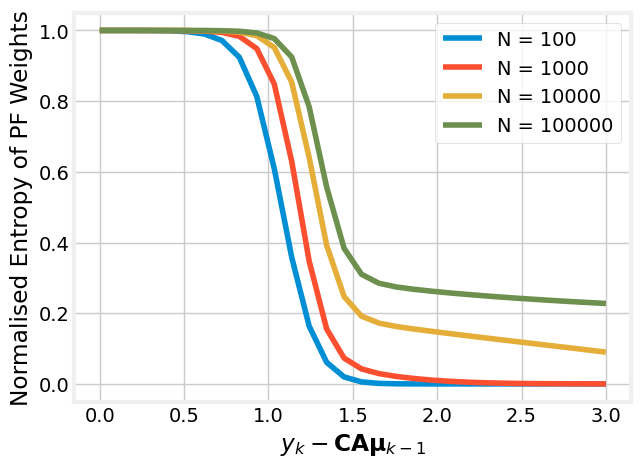
\includegraphics[width=12.0cm]{../plots/2__2__2__sample_impoverishment.png}
	\caption{Change in normalised entropy of PF weights as $\vt$ and $N$ are varied}
	\label{fig:2__2__2__sample_impoverishment}
\end{figure}
\end{document}